% Relatório - Trabalho 1 de FPPD: Jantar dos Filósofos
% Compilar:  pdflatex relatorio.tex   (ou no Overleaf)
% Números: média de 5 execuções de cada versão (resultados/resultados.csv).
\documentclass[11pt,a4paper]{article}

\usepackage[utf8]{inputenc}
\usepackage[T1]{fontenc}
\IfFileExists{lmodern.sty}{\usepackage{lmodern}}{}
\IfFileExists{brazil.ldf}{\usepackage[brazil]{babel}}{\usepackage[english]{babel}}
\usepackage[margin=2cm]{geometry}
\usepackage{booktabs}
\usepackage{tabularx}
\usepackage{array}
\usepackage{enumitem}
\usepackage{xcolor}
\usepackage{listings}
\usepackage{graphicx}
\usepackage{pgfplots}
\pgfplotsset{compat=1.16}
\usepackage[hidelinks]{hyperref}

\setlist{itemsep=2pt,topsep=4pt}
\setlength{\parskip}{4pt}
\setlength{\parindent}{0pt}
\newcolumntype{Y}{>{\raggedright\arraybackslash}X}

\lstset{basicstyle=\ttfamily\small, columns=fixed, keepspaces=true,
        frame=single, rulecolor=\color{gray!50}, backgroundcolor=\color{gray!5}}

% Marca de pendência (apagar quando os números finais entrarem)
\newcommand{\provisorio}{\textcolor{red!70!black}{\textbf{[PROVISÓRIO]}}}
\newcommand{\preencher}[1]{\textcolor{red!70!black}{\textit{#1}}}

\begin{document}

% =====================================================================
% PÁGINA 1: identificação, soluções, mecanismos e análise comparativa
% =====================================================================
\begin{center}
  {\Large\bfseries Trabalho 1 -- Concorrência e Sincronização:\\[2pt]
  O Problema dos Filósofos Jantando}\\[6pt]
  Fundamentos de Processamento Paralelo e Distribuído -- Profª.\ Eduarda Monteiro\\[2pt]
\end{center}

\begin{tabularx}{\textwidth}{@{}lY@{}}
\toprule
Grupo & R \\
Integrantes & Arthur Pimentel \textperiodcentered{} Raffaella Aranha \textperiodcentered{} Tiago Prudencio \\
Repositório Git & \preencher{link do repositório} (pasta \texttt{cmd/}, uma subpasta por versão) \\
\bottomrule
\end{tabularx}

\section*{Descrição das soluções e mecanismos de sincronização}

As quatro versões partem do exemplo sequencial do Moodle (\texttt{filo\_seq.go}) e mudam
só a forma de pegar os garfos. Todas usam 5 filósofos, 20 ciclos cada, 20\,ms para pensar
e 30\,ms para comer. Cada ciclo é: pensar $\rightarrow$ pegar os garfos $\rightarrow$ comer
$\rightarrow$ soltar os garfos.

\begin{tabularx}{\textwidth}{@{}>{\raggedright\arraybackslash}p{2.6cm}YYY@{}}
\toprule
\textbf{Versão} & \textbf{Como funciona} & \textbf{Mecanismo} & \textbf{Implementação em Go} \\
\midrule
V0 -- Sequencial & Um laço chama um filósofo de cada vez; ninguém disputa garfo &
  Nenhum (execução sequencial) & \texttt{Philosopher(j, i)} chamado dentro de dois \texttt{for} \\
\addlinespace
V1 -- Com deadlock & Cada filósofo é uma goroutine; todos pegam o garfo esquerdo e depois o direito &
  Exclusão mútua por garfo & Um \texttt{sync.Mutex} por garfo; \texttt{sync.WaitGroup} espera as goroutines \\
\addlinespace
V2 -- Sincronização excessiva & Igual à V1, mas um ``garçom'' só deixa um filósofo comer por vez &
  Semáforo binário global + mutex por garfo &
  Go não tem semáforo nativo: canal com buffer 1 (\texttt{chan struct\{\}}); enviar = P, receber = V \\
\addlinespace
V3 -- Concorrente & Igual à V1, mas todos pegam primeiro o garfo de menor número &
  Ordenação global dos recursos + mutex por garfo & \texttt{sync.Mutex} por garfo; o F5 troca a ordem (G0 antes de G4) \\
\bottomrule
\end{tabularx}

As métricas usam um \texttt{sync.Mutex} próprio, porque os 5 filósofos atualizam os mesmos
contadores ao mesmo tempo. O tempo é medido com \texttt{time.Now()} e \texttt{time.Since()}.

\section*{Análise comparativa}

A V3 foi a mais rápida (1,72\,s em média), 3,0 vezes mais rápida que a V0 (5,22\,s), porque
deixa 2 filósofos comerem ao mesmo tempo. A V2 não trava, mas o garçom limita a mesa a 1
filósofo comendo por vez. Por isso ela leva 3,15\,s e tem a maior espera pelos garfos:
102\,ms em média, contra 24\,ms na V3.

\begin{itemize}
  \item \textbf{V0:} tempo total = soma de todos os tempos ($20 \times 5 \times 50$\,ms $= 5$\,s).
        Espera zero, porque não há disputa.
  \item \textbf{V1:} travou nas 5 execuções, logo no 1.º ciclo, sem nenhum filósofo
        chegar a comer. Não serve como solução.
  \item \textbf{V2:} é correta e 1,7 vez mais rápida que a V0, porque os filósofos pensam em
        paralelo. Mas as refeições ficam em fila: $100 \times 30$\,ms $= 3$\,s, praticamente o
        tempo total medido.
  \item \textbf{V3:} é correta e tem o maior grau de concorrência possível com 5 garfos
        (2 comendo juntos). Ganha da V2 em tempo total e em espera.
\end{itemize}

% =====================================================================
% PÁGINA 2: tabela, gráfico, prints e evidência do deadlock
% =====================================================================
\newpage
\section*{Resultados experimentais}

Média de 5 execuções de cada versão; entre parênteses, o desvio padrão. A maior espera é a
maior observada nas 5 execuções.

\begin{center}
\small
\begin{tabular}{@{}lrrrcc@{}}
\toprule
\textbf{Versão} & \textbf{Tempo total} & \textbf{Espera média} & \textbf{Maior espera} & \textbf{Máx.\ comendo} & \textbf{Ciclos por} \\
 & \textbf{(ms)} & \textbf{(ms)} & \textbf{(ms)} & \textbf{juntos} & \textbf{filósofo} \\
\midrule
V0 -- Sequencial & 5218 ($\pm$35) & 0,0 & 0,1 & 1 & 20 em todos \\
V1 -- Deadlock & \multicolumn{5}{l}{travou nas 5 execuções (0 ciclos concluídos)} \\
\textbf{V2 -- Sinc.\ excessiva} & \textbf{3151 ($\pm$42)} & \textbf{102,0 ($\pm$1,5)} & \textbf{153,6} & \textbf{1} & 20 em todos \\
V3 -- Concorrente & 1719 ($\pm$61) & 24,3 ($\pm$0,6) & 75,0 & 2 & 20 em todos \\
\bottomrule
\end{tabular}
\end{center}

\begin{center}
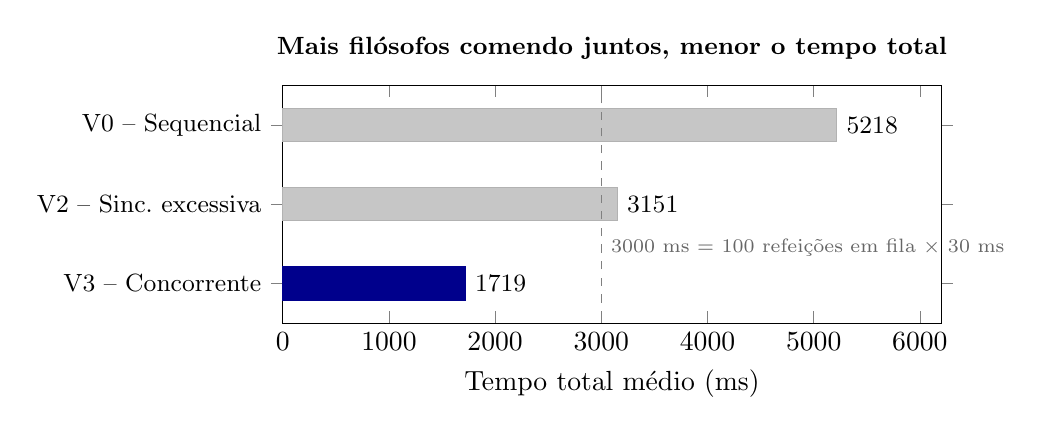
\begin{tikzpicture}
\begin{axis}[
  xbar, width=0.82\textwidth, height=4.6cm,
  bar width=12pt,
  xmin=0, xmax=6200,
  xlabel={Tempo total médio (ms)}, clip=false,
  scaled x ticks=false, xticklabel style={/pgf/number format/1000 sep={}},
  ytick={1,2,3}, ymin=0.5, ymax=3.5,
  yticklabels={V3 -- Concorrente, V2 -- Sinc.\ excessiva, V0 -- Sequencial},
  y tick label style={font=\small},
  nodes near coords, nodes near coords style={font=\small},
  every node near coord/.append style={/pgf/number format/1000 sep={}},
  title={Mais filósofos comendo juntos, menor o tempo total},
  title style={font=\bfseries\small},
]
\addplot[fill=gray!45, draw=gray!60, bar shift=0pt] coordinates {(5218,3) (3151,2)};
\addplot[fill=blue!55!black, draw=blue!55!black, bar shift=0pt] coordinates {(1719,1)};
\draw[dashed, gray] (axis cs:3000,0.55) -- (axis cs:3000,3.45);
\node[right, font=\scriptsize, text=gray!80!black, align=left] at (axis cs:3000,1.45)
  {3000 ms = 100 refeições em fila $\times$ 30 ms};
\end{axis}
\end{tikzpicture}
\end{center}

\vspace{-4pt}
{\small V0 e V2: 1 filósofo comendo por vez. V3: até 2 comendo juntos. A linha tracejada mostra
por que a V2 não fica abaixo de 3\,s: as 100 refeições acontecem uma de cada vez.}

\subsection*{Evidência do deadlock da V1}

Print de uma execução da V1 que travou. Cada coluna é um filósofo:
\texttt{T} = pensando, \texttt{G} = segurando um garfo, \texttt{E} = comendo.

\begin{minipage}[t]{0.49\textwidth}
\vspace{0pt}
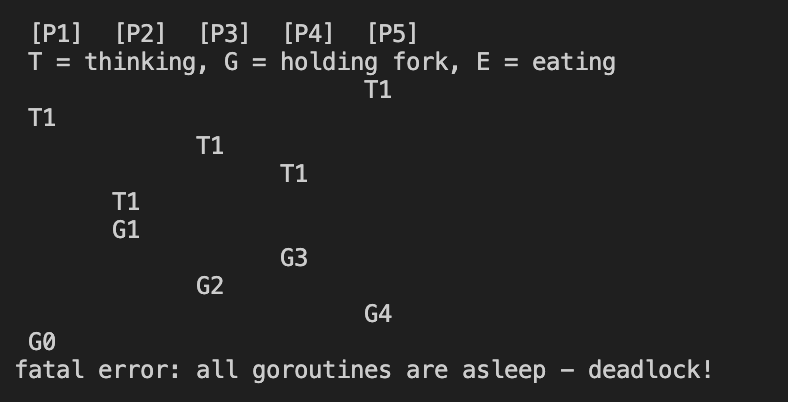
\includegraphics[width=\linewidth]{../resultados/prints/v1.png}
\end{minipage}\hfill
\begin{minipage}[t]{0.47\textwidth}
\vspace{0pt}
\small
\begin{tabular}{@{}cccc@{}}
\toprule
\textbf{Filósofo} & \textbf{Segura} & \textbf{Espera} & \textbf{Está com} \\
\midrule
P1 & G0 & G1 & P2 \\
P2 & G1 & G2 & P3 \\
P3 & G2 & G3 & P4 \\
P4 & G3 & G4 & P5 \\
P5 & G4 & G0 & P1 \\
\bottomrule
\end{tabular}

\smallskip
Nenhum filósofo chegou a comer: todos pegaram o garfo esquerdo e ficaram esperando o
direito. O runtime do Go detectou que todas as goroutines estavam bloqueadas e encerrou
o programa.
\end{minipage}

\subsection*{Saídas das execuções}

Final da saída de uma execução de cada versão que termina, no mesmo computador do print da V1.

\begin{minipage}[t]{0.32\textwidth}
\begin{lstlisting}[basicstyle=\ttfamily\scriptsize]
V0 took 5.217196709s
Average wait: 775ns
Max wait:     43.75us
Max eating together: 1
Cycles: [20 20 20 20 20]
\end{lstlisting}
\end{minipage}\hfill
\begin{minipage}[t]{0.32\textwidth}
\begin{lstlisting}[basicstyle=\ttfamily\scriptsize]
V2 took 3.129580542s
Average wait: 101.243705ms
Max wait:     124.283584ms
Max eating together: 1
Cycles: [20 20 20 20 20]
\end{lstlisting}
\end{minipage}\hfill
\begin{minipage}[t]{0.32\textwidth}
\begin{lstlisting}[basicstyle=\ttfamily\scriptsize]
V3 took 1.757039334s
Average wait: 23.847408ms
Max wait:     93.237583ms
Max eating together: 2
Cycles: [20 20 20 20 20]
\end{lstlisting}
\end{minipage}

% =====================================================================
% PÁGINA 3+: conclusão e respostas
% =====================================================================
\newpage
\section*{Conclusão}

Mais sincronização não significou mais desempenho. A V2, a mais sincronizada, é correta, mas
levou 3151\,ms. A V3 sincroniza só o necessário e levou 1719\,ms, 45\,\% menos. O que reduziu
o tempo total foi o grau de concorrência: 1 filósofo comendo por vez na V0 e na V2, 2 na V3.

\subsection*{1. Como funciona cada solução?}
A V0 executa um filósofo por vez, em laço. Na V1, na V2 e na V3, cada filósofo é uma goroutine
que repete 20 vezes: pensar, pegar os dois garfos, comer e soltar. As três diferem só na forma
de pegar os garfos: na V1, esquerdo e depois direito; na V2, pede antes a permissão do garçom;
na V3, primeiro o garfo de menor número.

\subsection*{2. Quais mecanismos de sincronização são utilizados?}
Exclusão mútua (um lock por garfo) na V1, na V2 e na V3. Na V2, também um semáforo binário
global. Na V3, ordenação global dos recursos. Em todas, uma barreira de término para o
\texttt{main} esperar os filósofos.

\subsection*{3. Como esses mecanismos são implementados em Go?}
O lock de cada garfo é um \texttt{sync.Mutex} (\texttt{Lock}/\texttt{Unlock}). A barreira é um
\texttt{sync.WaitGroup} (\texttt{Add}, \texttt{Done}, \texttt{Wait}). Go não tem semáforo na
biblioteca padrão, então o semáforo da V2 foi adaptado com um canal com buffer de 1:
\texttt{waiter <- struct\{\}\{\}} é o P (wait) e \texttt{<-waiter} é o V (signal).
A ordenação da V3 é só um \texttt{if} que troca a ordem dos dois garfos.

\subsection*{4. Por que ocorre deadlock na V1?}
Porque as quatro condições de Coffman estão presentes ao mesmo tempo:
\begin{itemize}
  \item \textbf{Exclusão mútua:} um mutex só pode estar com uma goroutine.
  \item \textbf{Segura e espera:} cada filósofo segura o garfo esquerdo enquanto espera o direito.
  \item \textbf{Sem preempção:} ninguém tira o garfo de outro; só o dono faz \texttt{Unlock}.
  \item \textbf{Espera circular:} P1 espera P2, que espera P3, \ldots, que espera P1 (tabela da página 2).
\end{itemize}
Isso aconteceu nas 5 execuções, sempre no 1.º ciclo, porque todos pensam o mesmo tempo e
chegam juntos aos garfos.

\subsection*{5. Como V2 e V3 evitam deadlock?}
A V2 quebra o ``segura e espera'': só quem tem a permissão do garçom pega garfos, então nunca
encontra um garfo ocupado. A V3 quebra a espera circular: como todos pegam primeiro o garfo de
menor número, um ciclo exigiria $G_a < G_b < \dots < G_a$, o que é impossível. Na prática, P1 e
P5 disputam o G0 como primeiro garfo, e quem perde espera sem segurar nada.

\subsection*{6. Existe possibilidade de starvation? Justifique.}
Na V0, não: a ordem é fixa. Na V2 e na V3, é teoricamente possível, porque nada garante a vez
de um filósofo. Nos experimentos ela não ocorreu: todos completaram 20 ciclos e a maior espera
foi 153,6\,ms na V2 (cerca de 5 refeições de 30\,ms) e 75,0\,ms na V3 (2,5 refeições). Isso acontece porque o
\texttt{sync.Mutex} do Go passa a atender em ordem de chegada quando uma goroutine espera mais
de 1\,ms, e porque cada filósofo pensa entre as refeições, dando vez aos vizinhos.

\subsection*{7. Qual solução apresentou maior tempo total de execução?}
A V0, com 5218\,ms, por ser sequencial. Entre as corretas e concorrentes, a V2 (3151\,ms).

\subsection*{8. Qual solução apresentou maior tempo de espera pelos recursos?}
A V2: 102,0\,ms em média e 153,6\,ms no pior caso, contra 24,3\,ms e 75,0\,ms na V3. A V1 fica
de fora, porque sua espera é infinita quando trava.

\subsection*{9. Quantos filósofos conseguiram comer simultaneamente em cada solução?}
V0: 1. V1: 0, porque travou nas 5 execuções antes de qualquer refeição. V2: 1. V3: 2, o máximo possível
com 5 garfos.

\subsection*{10. Qual foi o impacto da sincronização excessiva da V2?}
A V2 transforma as 100 refeições em uma fila: $100 \times 30$\,ms $= 3000$\,ms, quase todo o
tempo medido (3151\,ms). Comparada com a V3, foi 83\,\% mais lenta e teve espera média 4,2 vezes
maior, sem nenhum ganho de corretude.

\subsection*{11. A solução com maior sincronização foi a de melhor desempenho?}
Não. A V2 tem mais sincronização que a V3 (um semáforo global além dos mutexes) e foi pior em
todas as métricas de tempo: 3151\,ms contra 1719\,ms no total, e 102,0\,ms contra 24,3\,ms de
espera média. Sincronização garante corretude, mas cada trava a mais tira concorrência.

\subsection*{12. Qual é a relação entre o grau de concorrência e o tempo total?}
Quanto maior o grau de concorrência, menor o tempo total. Com 1 filósofo ativo por vez (V0),
5218\,ms. Com pensamento em paralelo, mas refeições em fila (V2), 3151\,ms. Com até 2 comendo
juntos (V3), 1719\,ms.

\section*{Ambiente de execução}

\begin{tabularx}{\textwidth}{@{}lY@{}}
\toprule
Linguagem e versão & Go \preencher{(saída de \texttt{go version} na máquina das medições)} \\
Sistema operacional & \preencher{(macOS: \texttt{sw\_vers})} \\
Processador & \preencher{(\texttt{sysctl -n machdep.cpu.brand\_string})} \\
Núcleos disponíveis & \preencher{(\texttt{sysctl -n hw.physicalcpu hw.logicalcpu})} \\
Parâmetros & 5 filósofos, 20 ciclos, pensar 20\,ms, comer 30\,ms (iguais nas 4 versões) \\
\bottomrule
\end{tabularx}

\begin{lstlisting}
go build -o bin/v3-concorrente ./cmd/v3-concorrente  # compila
./bin/v3-concorrente                                 # executa
go run ./cmd/v1-deadlock                             # compila e executa
go vet ./... && gofmt -l .                           # confere o codigo
./scripts/executar.sh                                # 5 execucoes de cada
\end{lstlisting}

\end{document}
